%!TEX output_directory = build
%!TEX copy_output_on_build = True
%!TEX options = --shell-escape
\documentclass[12pt, fleqn]{report}

%!TEX root = ./report.tex

\usepackage[top=3cm,bottom=3cm,left=3cm,right=3cm,headsep=10pt,a4paper]{geometry}

\usepackage{tikz} % Required for drawing custom shapes

% cite package, to clean up citations in the main text.
\usepackage{cite}

\usepackage{xcolor} % Required for specifying colors by name
\definecolor{ocre}{RGB}{243,102,25} % Define the orange color used for highlighting throughout the book

\usepackage{avant} % Use the Avantgarde font for headings
%\usepackage{times} % Use the Times font for headings
\usepackage{mathptmx} % Use the Adobe Times Roman as the default text font together with math symbols from the Sym­bol, Chancery and Com­puter Modern font
\usepackage{microtype} % Slightly tweak font spacing for aesthetics
\usepackage[T1]{fontenc} % Use 8-bit encoding that has 256 glyphs

\usepackage{calc} % For simpler calculation - used for spacing the index letter headings correctly


% Remove brackets from numbering in List of References
\makeatletter
\renewcommand{\@biblabel}[1]{\quad#1.}
\makeatother
\usepackage{url}

\usepackage{etoolbox}

%----------------------------------------------------------------------------------------
% TABLE OF CONTENTS
%----------------------------------------------------------------------------------------

\usepackage{titletoc}

\contentsmargin{0cm} % Removes the default margin

% Chapter text styling
\titlecontents{chapter}[1.25cm] % Indentation
{\addvspace{12pt}\large\sffamily\bfseries} % Spacing and font options for chapters
{\color{ocre!60}\contentslabel[\Large\thecontentslabel]{1.25cm}\color{ocre}} % Chapter number
{\color{ocre}}
{\color{ocre!60}\normalsize\;\titlerule*[.5pc]{.}\;\thecontentspage} % Page number

% Section text styling
\titlecontents{section}[1.25cm] % Indentation
{\addvspace{3pt}\sffamily\bfseries} % Spacing and font options for sections
{\contentslabel[\thecontentslabel]{1.25cm}} % Section number
{}
{\hfill\color{black}\thecontentspage} % Page number
[]

% Subsection text styling
\titlecontents{subsection}[1.25cm] % Indentation
{\addvspace{1pt}\sffamily\small} % Spacing and font options for subsections
{\contentslabel[\thecontentslabel]{1.25cm}} % Subsection number
{}
{\ \titlerule*[.5pc]{.}\;\thecontentspage} % Page number
[]



%----------------------------------------------------------------------------------------
% PAGE HEADERS
%----------------------------------------------------------------------------------------

\usepackage{fancyhdr} % Required for header and footer configuration

\pagestyle{fancy}
% \renewcommand{\chaptermark}[1]{\markboth{\sffamily\normalsize\bfseries\chaptername\ \thechapter.\ #1}{}} % Chapter text font settings
\renewcommand{\chaptermark}[1]{\markboth{\sffamily\normalsize #1}{}} % Chapter text font settings
\renewcommand{\sectionmark}[1]{\markright{\sffamily\normalsize\thesection\hspace{5pt}#1}{}} % Section text font settings
\fancyhf{}
\fancyhead[L]{\sffamily\normalsize\thepage}
\fancyhead[R]{\leftmark} % Print current chapter name

\renewcommand{\headrulewidth}{0.5pt} % Width of the rule under the header
\addtolength{\headheight}{2.5pt} % Increase the spacing around the header slightly
\renewcommand{\footrulewidth}{0pt} % Removes the rule in the footer
\fancypagestyle{plain}{\fancyhead{}\renewcommand{\headrulewidth}{0pt}} % Style for when a plain pagestyle is specified

% Removes the header from odd empty pages at the end of chapters
\makeatletter
\renewcommand{\cleardoublepage}{
\hbox{}
\vspace*{\fill}
\thispagestyle{empty}
\newpage}

%----------------------------------------------------------------------------------------
% CHAPTER HEADINGS
%----------------------------------------------------------------------------------------

\usepackage[explicit]{titlesec}

\newif\ifusechapterimage
\usechapterimagetrue
\newcommand{\thechapterimage}{}%
\newcommand{\chapterimage}[1]{\ifusechapterimage\renewcommand{\thechapterimage}{#1}\fi}

\definecolor{chapter_accent}{RGB}{90,90,90}

\newcommand\ChapterTitle[3]{%
  \begin{tikzpicture}[remember picture, overlay]
    \node at (current page.north west) {
      \begin{tikzpicture}[remember picture, overlay]
        \node [anchor = north west, inner sep = 0pt] at (0,0) {\ifusechapterimage\includegraphics[width=\paperwidth]{\thechapterimage}\fi};
        \draw [anchor = west] (\Gm@lmargin, -3cm) node [line width = 2pt, rounded corners = 15pt, draw=#2, fill=white, fill opacity = 0.9, inner sep = 15pt] {\strut\makebox[22cm]{}};
        \draw [anchor = west] (\Gm@lmargin+.3cm, -3cm) node {#1};
      \end{tikzpicture}};
  \end{tikzpicture}
  \vspace{#3}
}

\titleformat{name = \chapter, numberless}[block]
  {\normalfont\Large\sffamily\bfseries\color{black}}{}{0em}
  {\ChapterTitle{#1}{chapter_accent}{-3cm}}

\titleformat{name = \chapter}[block]
  {\normalfont\Large\sffamily\bfseries\color{black}}{}{0em}
  {\ChapterTitle{\thechapter.\ #1}{chapter_accent}{-2cm}}


%----------------------------------------------------------------------------------------
% SECTION HEADINGS
%----------------------------------------------------------------------------------------

\definecolor{section_accent}{RGB}{90,90,90}

\newcommand\SectionTitle[3]{
  \begin{tikzpicture}[remember picture, overlay]
    \draw [anchor = west] (-.5cm, 0) node [rounded corners = 10pt, fill = #1, inner sep = 10pt] {\strut\makebox[2.5cm]{}};
    \draw [anchor = west] (1cm, 0) node {\color{white}{\large#2}};
    \draw [anchor = west] (3cm, 0) node {#3};
  \end{tikzpicture}
}

\titleformat{\section}
  {\normalfont\Large\sffamily\bfseries\color{black}}{}{-3cm}
  {\SectionTitle{section_accent}{\thesection}{#1}}
 % defines page geometry, table of contents layout, and section and chapter headings

\usepackage{amsmath, amssymb} % useful for mathematical formulas and symbols

\usepackage[english]{babel} % English language/hyphenation

\usepackage{graphicx} % including graphics, such as pdfs
\graphicspath{{./figures/}{./figures/images/}{./headers/}{./plots/}}

\usepackage{shellesc}
\usepackage{pgfplots}
\usepackage{grffile}
\pgfplotsset{compat=newest}
\usetikzlibrary{plotmarks}
\usetikzlibrary{arrows.meta}
\usepgfplotslibrary{patchplots}
\usetikzlibrary{external}


% Bold the 'Figure #' in the caption and separate it with a period
% Captions will be left justified
\usepackage[labelfont=bf,labelsep=period,justification=raggedright]{caption}
\usepackage{subcaption} % add subfloats
\usepackage{wrapfig} % wrap text around figure
\usepackage{placeins} % create float barriers


\usepackage{enumitem} % Customize lists
\setlist{nolistsep} % Reduce spacing between bullet points and numbered lists


\usepackage{booktabs} % Required for nicer horizontal rules in tables
\usepackage{longtable}
% \usepackage{tabularx}
% \newcolumntype{Y}{>{\centering\arraybackslash}X}


\usepackage{setspace}
\onehalfspacing
\parskip = 11pt % adds vertical space between paragraphs

\usepackage{nomencl}
\makenomenclature

% \usepackage[unicode=true]{hyperref}

\usepackage{lipsum}
\usepackage{blindtext}


\begin{document}

% Title Page
\begingroup
\thispagestyle{empty}
\tikzsetnextfilename{title_page}
\begin{tikzpicture}[remember picture,overlay]
  \node[inner sep=0pt] (background) at (current page.center) {
\includegraphics[width=\paperwidth]{background}};
  \draw (current page.center) node [fill=ocre!30!white,fill opacity=0.6,text opacity=1,inner sep=1cm]{\Huge\centering\bfseries\sffamily\parbox[c][][t]{\paperwidth}{\centering Surgitouch\\[15pt] % Book title
  {\Large A 2 Degree of Freedom Haptic Joystick}\\[20pt] % Subtitle
  {\huge Dr. John Smith}}}; % Author name
\end{tikzpicture}
\vfill

\endgroup


\begin{abstract}
This is a really good report, promise. Please give us an A. Pretty please.
\end{abstract}

\usechapterimagefalse

\nomenclature{$c$}{Speed of light in a vacuum inertial frame}
\nomenclature{$h$}{Planck constant}

\printnomenclature


\pagestyle{empty}
\tableofcontents
\pagestyle{fancy}

\usechapterimagetrue
\chapterimage{default.pdf}

\chapter{Example} \label{cha:example}
\section{Text} \label{sec:text}
\lipsum[1-7]
% section text (end)
\section{Math Section} \label{sec:math_section}
\blindmathpaper
% section math_section (end)



\chapter{Introduction}\label{cha:introduction}
\section{Background}
\label{sec:background}
Scope of the project, the project will be used by the Mechatronics in medicine department at Imperial college for the STING project. Give details of this. Then the wider scale overall aim of project is to be incorporated into the international EDEN 2020 project.
% section background (end)

\section{Team Roles}
\label{sec:team_roles}

% section team_roles (end)

\section{Objectives}
\label{sec:objectives}
What the client wants.
% section objectives (end)


\section{Structure of Report}
\label{sec:structure_of_report}
Explain the order of the report: Design Section. Make, Test.
% section structure_of_report (end)


% \chapter{Literature Review}\label{cha:lit_review}
% %!TEX root = ../report.tex
\section{Joystick Review} % (fold)
\label{sec:joystick_review}

Joysticks are devices which allow a user to control a point in a "virtual map" to get a certain output (be it the point moving a component in real life, or purely virtually) based on the input to the joystick (ie. its current orientation). Simple joysticks may be used for applications from gaming simulators to basic telemanipulation to RC control. In this report it is joysticks with force feedback that are being looked at.

Haptic joysticks give the user feedback based on their inputs, an example being mechanical aircraft joysticks which give the pilot feedback based on the direction of their flight path. Without this feedback, it would be comparable to driving a racing car without the feeling of the road, an incredibly dangerous experience. In commercial use however, force feedback joysticks are limited, especially at a low price point, due to their previous limited applications. The use in medicinal technology is on the rise such that now further research and development in them is required.


\subsection{Joystick Mechanisms} % (fold)
\label{sub:joystick_mechanisms}

There are many types of joystick dependent on the necessary application. Varying from a single degree of freedom which could purely control speed, to 2DOF for dual axis positional control, and upwards. The mechanisms for these varies massively for different degrees of freedom and different uses. A single axis joystick will be a simple rotation, dual axis rotation about two axes, etc. Naturally the more axes, the more complex the system and the higher some factors are, ie inertia, and noise levels.

% subsection joystick_mechanisms (end)

\subsection{Button Joystick} % (fold)
\label{sub:button_joystick}

Perhaps the simplest type, the button joystick relies on four pressure sensitive contacts which can be pressed either alone, or together to give a variety of responses. These were used in early games consoles and basic RC controllers. An example can be seen in Figure~\ref{fig:button_joystick}.

\begin{figure}
  \centering
  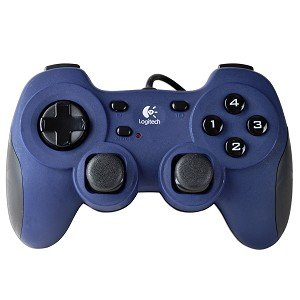
\includegraphics[width=0.5\textwidth]{button_joystick.jpg}
  \caption{Button Joystick}
  \label{fig:button_joystick}
\end{figure}

% subsection button_joystick (end)

\subsection{Continuous "track" Joystick} % (fold)
\label{sub:continuous_joystick}

The track, or gimbal joystick is the basis of almost all modern games controllers. The joystick itself pivots about a ball mechanism and extends beyond it. The extension rests in two tracks connected to potentiometers, which, when they are moved are able to give a reading of the location of the joystick in space. See Figure~\ref{fig:continuous_joystick} for further details.

\begin{figure}
  \centering
  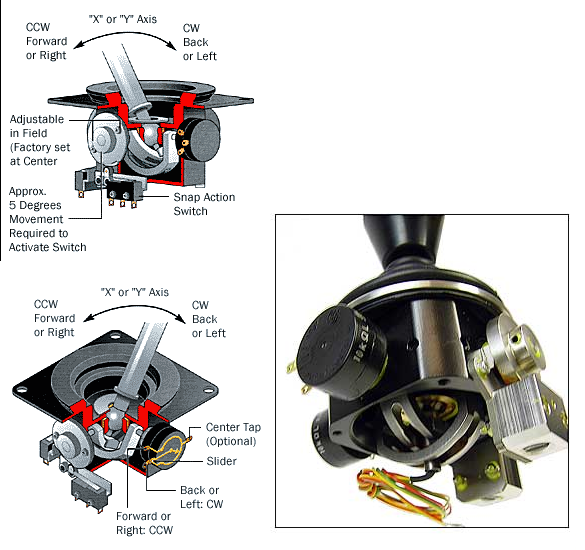
\includegraphics[width=0.5\textwidth]{continuous_joystick.png}
  \caption{Continuous Joystick}
  \label{fig:continuous_joystick}
\end{figure}

This method is compact, but has complex moving parts and can suffer from higher inertia. It is however very cheap and easy to produce. A mechanical two axis system is of most relevance to us due to its price point, and ease of use.

% subsection continuous_joystick (end)

\subsection{Accelerometer and sensor based "position tracking"} % (fold)
\label{sub:accelerometer_and_sensor_based}

A slightly newer form of controller, adopted in many forms of controllers due to its ability to be used in any position and multiple degrees of freedom. Perhaps the most mainstream use of this is in the Nintendo Wii games joystick. These use motion control and accelerometers to measure how far they have moved and in which direction in space, giving them an awful lot of freedom for movement in space. Whilst they can be accurate, expensive position sensors are normally needed, as well as a good form of calibration. These can suffer from a number of downfalls, most notably the trick of learning how to carefully use them in complex environments. Limiting the number of degrees of freedom per joystick can be seen as advantageous due to being simpler to control. They can also suffer from low accuracy and repeatability of position if there is any interference.

It is also possible to have external sensors measure movements of a person in space, ora person holding set instruments in space. These work by a light source illuminating the object, and sensors measuring the distance the light travels to each part of the object. These points are then interpreted and mapped in relevant software. Whilst relatively accurate, for very fine movements, the precision of a system like this can falter. It is also not possible to get force feedback from a design like this.


% subsection accelerometer_and_sensor_based (end)

\subsection{Trackball} % (fold)
\label{sub:trackball}

Another type of 2D joystick, however also quite difficult to control.
As depicted in Figure~\ref{fig:trackball}, trackballs protrude from the casing and are able to rotate in any direction, and move continuously allowing for fast movement.
The position is measured by small wheels on the inside of the casing that move with the ball due to friction.
It is possible to add haptic feedback to a system like this, although due to the necessary size of the positionsensing wheels, hard to get a desired feedback.

\begin{figure}
  \centering
  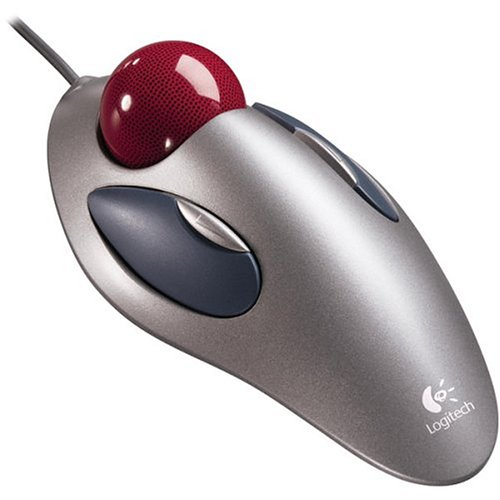
\includegraphics[width=0.5\textwidth]{trackball.jpg}
  \caption{Trackball}
  \label{fig:trackball}
\end{figure}

% subsection trackball (end)

\subsection{Summary} % (fold)
\label{sub:summary}

There are in fact many more forms of mechanisms, both complex and simple than the ones discussed, however these are viewed as the most relevant in the scope of this project due to the desire for a minimal inertia, cost friendly and very precise system. More research into an adequate design is shown in SECTION.

% subsection summary (end)

% section joystick_review (end)

\section{Haptic Technologies} % (fold)
\label{sec:haptic_technologies}

The force feedback is equally as important as the mechanism for this project, and researched had to be undertaken to see the quality of what is currently available. As can be seen, for our price point and application, the literature discovered is quite limited.

\subsection{High End - Da Vinci system, Omni Controller} % (fold)
\label{sub:high_end_da_vinci_system}

% subsection high_end_da_vinci_system (end)

\subsection{Mid Range - Haptic Cow, MR System} % (fold)
\label{sub:mid_range_haptic_cow_mr_system}


% subsection mid_range_haptic_cow_mr_system (end)

\subsection{Low End - Gaming devices, flight joysticks, Hapkit} % (fold)
\label{sub:low_end_gaming_devices_flight_joysticks_hapkit}

% Haptic Cow, Virtual reality, gaming devices,  and geomagic interfaces used for 3D designing. At the moment the mechatronics department is using a piece like this but it is very expensive and large -> therefore leading onto the requirement of something smaller with more basic functionalities.
% Then onto research papers and patented designs of joystick mechanisms.
% Input MR haematoglogical paper which we based our gimbal mechanism on.
% Input awesome paper medler found with springs. (explain reasons why this may be a little too optimistic for us to produce with budget limitations / can’t copy patented design)
% 3) Others that are similar to ours, other projects\\
%     Cool paper with the patent. Hapkit ; two papers I have bookmarked; first one we found with MR, but same mechanism\\
% 4) Professional ones;\\
%     Omni controller; Da vinci controller\\


% subsection low_end_gaming_devices_flight_joysticks_hapkit (end)

% section haptic_technologies (end)

% \chapter{Technincal Background}\label{cha:tech_background}
% %!TEX root = ../report.tex

\section{Force Feedback Applications} % (fold)
\label{sec:force_feedback_applications}



% section force_feedback_applications (end)

\section{Control Theory and System design} % (fold)
\label{sec:control_theory_and_system_design}


% section control_theory_and_system_design (end)

\section{Introduction to Microcontrollers and Arduinos} % (fold)
\label{sec:introduction_to_microcontrollers_and_arduinos}

Microcontrollers are the chief element of any embedded application. A microcontroller is composed of several different elements; a processing unit (CPU) to handle execution of tasks, memory, input / output (I/O) ports and timers. As well as any peripherals, such as analogue to digital converters (ADCs) or serial communication (UART) that can add additional functionality.

The Ardunio framework is based on the popular range of Atmel AVR chips, and provides a simpler starting point for the development of an embedded application. Ardunio provide many libraries which simplify working with particular peripherals and any I/O, enabling a quicker development time, particularly during the concept phase.

% section introduction_to_microcontrollers_and_arduinos (end)

\section{Robot Operating Systen} % (fold)
\label{sec:robot_operating_system}

The Robot Operating System (ROS) is a software suite designed to make producing complex robotics software simpler. It consists of a large collection of tools, libraries, drivers, and packages to do this. ROS encourages collaboration between research institutes through its highly modular framework. For example, say an institute specialises in mapping environments, and produces a ROS package that does this brilliantly, another institute can use this package to navigate through indoor spaces using these maps without having to develop a mapping system themselves. Further examples include a package to retrieve and process images from a camera device, or a package for a specific encoder or motor to enable simpler control.


A typical ROS application will consist of various "nodes", which perform specific tasks. ROS typically communicates between nodes over topics. Topics are named buses over which nodes exchange messages, if a node is interested in data of a topic it \emph{subscribes} to that particular topic, whereas nodes which generate data \emph{publish} data to the relevant topic (@ROS Wiki). ROS also has another method of communication between topics called services. These differ from messages in that a callback is issued, these services work in a similar way to a function call in a program, data is sent to a particular node which has advertised a service, a calculation is then carried out, or data obtained and processed, and is then sent back to the node which initially sent the data.

% section robot_operating_system (end)

% \chapter{Design Parameters}\label{cha:design_params}
% Nothing here.

% \chapterimage{control_section.pdf}
% \chapter{Electronics Development}\label{cha:electronics_dev}
% \section{Motor Selection}
\label{sec:motor_selection}

% section motor_selection (end)

\section{Controller Selection}
\label{sec:controller_selection}

% section controller_selection (end)

\section{Software Choice}
\label{sec:software_choice}

% section software_choice (end)

\section{PID Control}
\label{sec:pid_control}

Here is some stuff about PID control

\begin{figure}
  % This file was created by matlab2tikz.
%
%The latest updates can be retrieved from
%  http://www.mathworks.com/matlabcentral/fileexchange/22022-matlab2tikz-matlab2tikz
%where you can also make suggestions and rate matlab2tikz.
%
\definecolor{mycolor1}{rgb}{0.00000,0.44700,0.74100}%

\tikzsetnextfilename{linear_force_location}
\centering
\begin{tikzpicture}
\begin{axis}[
  % width=6.127in,
  width=0.5\textwidth,
  % height=4.279in,
  at={(1.028in,0.578in)},
  scale only axis,
  xmin=-50,
  xmax=50,
  xlabel style={font=\color{white!15!black}},
  xlabel={Shaft position ($^\circ$)},
  ymin=0,
  ymax=1.2,
  ylabel style={font=\color{white!15!black}},
  ylabel={Force (N)},
  axis background/.style={fill=white},
  % title style={font=\bfseries},
  % title={Linear force - location relationship},
]
\addplot [color=mycolor1, line width=1.5pt, forget plot]
  table[row sep=crcr]{%
-50	1.19\\
0	0.109999999999999\\
50	1.19\\
};
\end{axis}
\end{tikzpicture}%
\end{figure}

% section pid_control (end)

\section{Placement of Electronic Components}
\label{sec:placement_of_electronic_components}

% section placement_of_electronic_components (end)


% \chapter{Mechanism Development}\label{cha:mechanism_dev}
% %!TEX root = ../report.tex

\section{Initial Design Concepts} % (fold)
\label{sec:initial_design_concepts}

\subsection{2 DOF Mechanism} % (fold)
\label{sub:2_dof_mechanism}

\begin{wrapfigure}{R}{0.4\textwidth}
  %!TEX root = ../report.tex
% Set the plot display orientation
% Syntax: \tdplotsetdisplay{\theta_d}{\phi_d}
\tdplotsetmaincoords{60}{110}

% Start tikz-picture, and use the tdplot_main_coords style to implement the display
% coordinate transformation provided by 3dplot.
\centering
\begin{tikzpicture}[scale=2,tdplot_main_coords,xshift=2cm]

% Set origin of main (body) coordinate system
\coordinate (O) at (0,0,0);

% Draw main coordinate system
\draw[thick,->] (0,0,0) -- (1,0,0) node[anchor=north east]{$x$};
\draw[thick,->] (0,0,0) -- (0,1,0) node[anchor=north west]{$y$};
\draw[thick,->] (0,0,0) -- (0,0,1) node[anchor=south]{$z$};

%Draw the arcs on each theta plane
%The first position is obvious since we are in the x-y plane and rotating around the z-axis.
%The anchor already went crazy, north is pointing downwards...
\tdplotdrawarc[->,color=black]{(0,0,0.7)}{0.1}{0}{350}{anchor=south west,color=black}{$c$}
%We move to the z-x axis
\tdplotsetthetaplanecoords{0}
%Notice you have to tell tiks-3dplot you are now in rotated coords
%Since tikz-3dplot swaps the planes in tdplotsetthetaplanecoords, the former y axis is now the z axis.
\tdplotdrawarc[tdplot_rotated_coords,->,color=black]{(0,0,0.7)}{0.1}{110}{460}{anchor=south west,color=black}{$b$}
\tdplotsetthetaplanecoords{-90}
%Once again we swaps the planes. I don't know why it's working like this but we turn backwards
%so the arrow turns in the positive direction.
\tdplotdrawarc[tdplot_rotated_coords,->,color=black]{(0,0,0.7)}{0.1}{120}{470}{anchor=south west,color=black}{$a$}
% If you turn the theta plane  of 90 degrees position and rotation are inverted.
%\tdplotsetthetaplanecoords{90}
%\tdplotdrawarc[tdplot_rotated_coords,->,color=black]{(0,0,-0.7)}{0.1}{470}{120}{anchor=south east,color=black}{roll}
\end{tikzpicture}
  \caption{3D Axis visualisation}
  \label{fig:3d_axis}
\end{wrapfigure}

Three main mechanisms were considered for a device that could rotate in two ($a$ and $b$)
degrees of freedom but maintain constrained in the others ($x$, $y$, $z$, and $c$).
Each design was examined carefully on whether or not an additional degree of
freedom in $c$ could be incorporated into the mechanism as an area for future
development of the final prototype, however, three degrees of freedom was not
vital.

The three mechanisms consisted of:

\begin{itemize}
  \item A mouse-ball with two perpendicular driving rollers
  \item A gimbal rotating around two perpendicular shafts
  \item A ball-in-socket moved by perpendicular sets of tensioning cables
\end{itemize}

{\color{red}Insert diagrammatic explanations of each + include explanations of pros/cons of each.
Then go onto choice of 2.}

% subsection 2_dof_mechanism (end)

\subsection{Force Feedback Deployment Measures} % (fold)
\label{sub:force_feedback_deployment_measures}

For a gimbal mechanism, a resistance torque applied on each perpendicular shaft is
the basis of the force feedback on the user’s end of the joystick. With more
research into joystick designs a few different methods were considered and
calculations made to prove the validity of each one. Research into mechatronics
and haptics papers have shown the use of electro-rheological (ER) and magneto-rheological (MR) fluids which
can be used to provide variable force feedback by varying electric or magnetic
fields, respectively. These mechanisms are highly advanced and the technology
required to do this would not only make the joystick assembly much larger, but
more complex to manufacture and out of range of the project budget. The various designs do all however make use of DC motors, brakes, clutches, gears, belts and pulleys as means of deploying force feedback. Hence, taking away some ideas from the mechanism functionalities the following design concepts for a smaller, lower-budget, easily manufacturable device were investigated:

\begin{itemize}
  \item Bike cable braking system to apply resistance torque onto shaft
  \item Linear actuators that apply variable pressure and resistance torque similar to a frictional clutch
  \item Direct motor on shaft
  \item Geared motor with clutch engagement/disengagement
\end{itemize}

Insert drawings of each concept and evaluate reasons for choice of concept (c).

% subsection force_feedback_deployment_measures (end)

\subsection{Choice of Driving System} % (fold)
\label{sub:choice_of_driving_system}


From preliminary tests in order to get a full range of force feedback the desired maximum
torque should lie within the range of 62-79 mNm, with a minimum torque in the range of 5-8 mNm,
although depending on choices of motor, the feedback range can be subject to change.
Additionally important specifications of the motor are inertia and size. From the PDS the whole
mechanism must have extremely low inertia. Because the main source of inertia is in the rotary
mechanism and windings of motor, this was a critical part to look into. More details of the
motor selection process are found in the next section on electronics development. For the next
two sections 6.3 and 6.4, the relevant parameters of the motors chosen for the final prototype,
used for designing the mechanism, are:

% \begin{longtable}[h]{@{}ll@{}}
%   \toprule
%   Nominal torque  & $T_{\text{nom}}$    &   45.5 mNm    \tabularnewline
%   Stall torque    & $T_{\text{stall}}$  &   212 mNm     \tabularnewline
%   Rotor inertia   & $J_{\text{motor}}$  &   45.3 gcm²   \tabularnewline
%   Outer Diameter  & $\Theta_{O}$        &   240 g       \tabularnewline
%   Length          & $L_{\text{motor}}$  &   61.5 mm     \tabularnewline
%   \bottomrule
% \end{longtable}

% subsection choice_of_driving_system (end)

% section initial_design_concepts (end)

\section{Failure Analysis and Design Optimisation} % (fold)
\label{sec:failure_analysis_and_design_optimisation}

One of the main specifications of this project was to produce a prototype that was small
and portable. From the PDS the aim is to get the whole assembly to a size smaller than 200 x 200 x 200 mm. With motors must be placed at the end of perpendicular shaft leaving around 140 x 140 mm x 200 mm of space to work with for design of the gimbal.
For motor-driven shafts with opposing forces applied by the user’s fingers at the joystick end, there are various forces and moments which must be transferred along shafts and via the gimbal mechanism between components. Therefore, all parts in the gimbal mechanism must be designed to cope with these without failure.
Two other modes of failure which are also possible are fatigue due to repeated loading and thermal overheating of electrical components (discussed in later section on electronics development and final prototype), however due to the low duty cycle and vibrations fatigue is negligible.

\subsection{Main Design Iterations} % (fold)
\label{sub:main_design_iterations}

\paragraph{Initial Prototype design} % (fold)
\label{par:initial_prototype_design}

General overview of the setup Plan view below: Two perpendicular shafts, two degrees of freedom of rotation about x and y axes, force feedback in each direction applied by perpendicular motors attached directly to shafts. Reduced inertia by having as little things attached to the motor shafts as possible. Encoders attached to opposite end of motor where shafts are not under applied torsion and are free to rotate. Position in the overall work-space will be defined by combined angular displacement measurements from perpendicular encoders.

The main parts to design are in the central box - the gimbal mechanism. Design iterations and the reasonings for them will be outlined in this section.

% paragraph initial_prototype_design (end)

\paragraph{Initial Prototype Mechanism} % (fold)
\label{par:initial_prototype_mechanism}

Gimbal curves upwards, so motor shafts can sit as low as possible and the joystick cover rests at a height above the radius of the gimbal. The joystick is attached to the main shaft via a Delrin piece, so when the joystick rotates about the gimbal axis there is low friction rubbing of Delrin against aluminium shaft (as opposed to using and metal piece). A bushing would be placed in the hole between ptfe piece and the bolt which feeds through the shaft, so that there is less frictional resistance to rotation on this face. The gimbal component consists of a curved piece and two shafts with external threads secured to the curved piece by nylon-insert lock nuts, to resist turning, so the curved piece moves together with the shafts. A slot-track is machined through the curved piece for the joystick to move through. A nylon or PTFE collar will be placed around the joystick shaft to reduce friction and provide smooth gliding of the joystick through the slot-track.

When manufacturing the prototype, issues of flexibility of PTFE meant that machining to the high tolerance necessary was difficult. The flexibility also was not acceptable for the function of the shaft because of increased mechanical play at the joystick end. The stiffness of this part therefore needed to be increased greatly.

After further inspection and testing of prototype it was decided that if the nuts were placed concentric along the axis of rotation of the pieces it was holding together, it would eventually come loose enough incurring even more mechanical play of the joystick. This was a major issue when it came to testing the preliminary prototype, hence a number of alternatives were investigated.

% paragraph initial_prototype_mechanism (end)

\paragraph{Gimbal Design Iterations} % (fold)
\label{par:gimbal_design_iterations}

(a \& b) Flanged curved piece CNC milled with two parts separately turned down in the lathe. Each part with holes drilled into them and countersunk bolts to leave a sleek looking face and hold the parts together.

(a) Using 4 eccentric screws, hence providing no room for vertical or horizontal play. However due to the small dimensions of this piece the area of piece to drill is less than 20 x 20 mm, meaning that the size of the holes must be very small in order for the adjacent nut and washer fittings not to interfere with each other in addition to the assembly the bolt heads must be small enough to fit in next to the shaft.

(b) Using 2 eccentric screws of slightly larger diameter, this may add increased vertical instability however the flange should support the shaft pieces and counteract this. However, the bolts must be less than M3 in diameter, and because the applied torque from motors will be transmitted to the joystick directly through the bolts, while some stress relief comes from the flange, the likelihood of shearing of the bolts over a long period of use is relatively high.

(c) Laser-cutting two parallel tracks from acrylic and fixing to aluminium side shafts which can withstand torsion. The Acrylic-PTFE surface is extremely low friction providing a smooth motion of joystick through tracks. However fixing acrylic to metal would not be possible with glue because of its surface finish, and drilling of holes for fixtures adds more stress concentrations into the already relatively lower-strength acrylic. A prototype version for the side-tracks was trialled for strength and failed under applied torsion. An extremely thick sheet of acrylic would be necessary and would not fall in line with the size constrictions of the assembly.

(d) 3D printing a wholly combined piece so there are no fixtures and stresses are transferred directly through the body. This is a much more reliable design, but requires 3D printing of a material with stiffness comparable to metals or metal sintering. When inquiring about a metal sintered sample the price quote started at (euros)400 from FKM laser sintering which was out of the budget for mechanism materials. A prototype was 3D printed from ABS, to trial the mechanism and dimensions. However after further stress analysis outlined in the next section 6.3.2 the order of GPa is required for this application so any plastic component cannot be used (ABS has a flexural stiffness in the order of MPa).

(e) The final choice was similar to all the above, using the same dimensions as the (a) and (b) but the whole piece concept of (d), the metal pieces would be welded together with no holes. Using lightweight aluminium, which welds much better than steel, the final piece would be much stronger than any of the above choices.


% paragraph gimbal_design_iterations (end)

\paragraph{Joystick Design Iterations} % (fold)
\label{par:joystick_design_iterations}

The original joystick design consisted of a delrin block with holes drilled across for the main shaft pin, and a hole drilled into the top for the joystick to screw into and be tightened up with a nut. After manufacturing a prototype piece, it was evident that even though delrin had a high stiffness in comparison to other plastics, in this shape configuration the stiffness was still not high enough, this is validated by stress analysis of this part in section 6.3.2.4. Another issue with this set-up was that there was a large amount of mechanical play because the fixing of joystick perpendicular to top face of delrin block was not completely rigid.

To fix the flexing issue a material of higher flexural modulus was required, so aluminium was used instead for this part. A special flanged bearing setup was used to solve the frictional issues and this will be shown in more detail in section 6.2.4. To solve the issue of mechanical play, instead of having two separate parts, it would be manufactured from one piece of metal - slightly more complex to machine, but this would improve rigidity vastly.

The diagram below shows the development of the joystick. The final piece with the gimbal part sitting underneath the origin of rotation, this allows for more space on the top so the complexity of the casing cover could be reduced to a flat top. This also allowed for joystick length reduction - reducing overall torque necessary to produce the same force feedback for user.

% \begin{longtable}[h]{@{}ll@{}}
%   \caption{Friction Coefficients}
%   \toprule
%   Aluminium         & XX    \tabularnewline
%   PTFE              & XX     \tabularnewline
%   Delrin            & XX   \tabularnewline
%   Nylon             & XX       \tabularnewline
%   Other plastics    & XX     \tabularnewline
%   \bottomrule
% \end{longtable}

Aluminium seizes on contact, so considered using aluminum-aluminum with lube - Coefficient of friction increases over time until complete fusion of parts. Long-term not great. High maintenance lubrications.

Instead we used an flanged support so the faces are not touching.
Dual friction PTFE plates surrounding both parts, but requires complex adherence to part.
Otherwise Teflon spray coating.

PTFE will rub away over time and produce an even smoother motion, although it will reach a point where it has rubbed away so much that the piece will require replacement due to increased mechanical play.


% paragraph joystick_design_iterations (end)

% subsection main_design_iterations (end)

% section failure_analysis_and_design_optimisation (end)

\section{Ergonomics} % (fold)
\label{sec:ergonomics}

\subsection{Joystick Handle} % (fold)
\label{sub:joystick_handle}

Nada

% subsection joystick_handle (end)

\subsection{Wrist Support} % (fold)
\label{sub:wrist_support}

The surgitouch will be used for extended periods of time during surgery, meaning care must be taken to ensure that the surgeon’s wrist rests in a comfortable and healthy position to avoid muscular strain. Incorrect support of the arm and wrists can cause excessive pressures on the delicate tendons on the underside of the wrists, leading to tenosynovitis (inflammation of the sheath surrounding tendons) and carpal tunnel syndrome. According to the American Occupational Safety and Health Administration, the following things must be considered when choosing a rest:

\begin{itemize}
  \item “Your hands and wrists should move freely and be elevated above the wrist/palm rest. When resting, the pad should contact the heel or palm of your hand, not your wrist.
  \item Reduce bending of the wrists by adjusting other workstation components (chair, desk, keyboard) so the wrist can maintain an in-line, neutral posture.
  \item Provide wrist/palm supports that are fairly soft and rounded to minimize pressure on the wrist. The support should be at least 3.8 cm (1.5 inches) deep.”
\end{itemize}

Using these guidelines, a few ideas were sketched out as shown below. Care was taken to place the rest such that it could be used by both left and right handed surgeons.

As opposed to the joystick grip, which was specified for the diameter of our joystick and thus needed to be 3D-printed, arm rests are a fairly common product and can be bought from retailers. Therefore, the guidelines and sketches were used to buy a rest which met our requirements:

% subsection wrist_support (end)

% section ergonomics (end)

% \chapter{Final Prototype}\label{cha:final_prototype}
% \section{Gimbal Mechanism}
\label{secgimbal_mechanism}

Design aspects of every part we made/used and how they all interact.

Minimum allowable sizes (stress analysis – max forces applied). Also maximum sizes due to lack of fit / clashes of moving mechanism.

Friction Analysis and low intertia

% section gimbal_mechanism (end)

\section{Electrical Circuitboards}
\label{secelectrical_circuitboards}

Picture of boards with diagrammatic explanations

% section electrical_circuitboards (end)

\section{Haptic Feedback Implementation (Software)}
\label{sechaptic_feedback_implementation_}

Flow Charts

% section haptic_feedback_implementation_ (end)

\section{Cooling Considerations}
\label{seccooling_considerations}
Simply put two fans and holes in sidewalls of main casing to keep all components (motor, controller and arduino cool).
Limit device use time, so that motors do not over heat. For longer usage times a more expensive and efficient cooler is required because the motors heat up to a large extent.

Motors left in open air and the plastic insulated parts are attached to the main housing via screws. A slotted base support is used to hold weight of the motor and reduce stresses at the main mechanism housing (although stresses are small already, a good idea to add support to reduce even more, to point where screws simply orient motor in correct direction and do not support the weight of it - in case of vibrations of motor and repeated cyclic loading causing fatigue failure of housing due to cyclic bending stresses).

% section cooling_considerations (end)

\section{Casing and Ergonomic Design}
\label{seccasing_and_ergonomic_design}

% section casing_and_ergonomic_design (end)

\section{Placement of Electronic Components}
\label{secplacement_of_electronic_components}

Map out with dimensions the base of housing. Show different coloured wires to/from each electronic component. Consider different ways of tidying wires and choose an option.

%section placement_of_electronic_components (end)

% \chapter{Manufacturing}\label{cha:manufacturing}
% %!TEX root = ../report.tex

\section{Manufacturing Timeline} % (fold)
\label{sec:manufacturing_timeline}

Picture goes here

% section manufacturing_timeline (end)

\section{Engineering Drawings} % (fold)
\label{sec:engineering_drawings}

% section engineering_drawings (end)

\section{Manufacturing Process} % (fold)
\label{sec:manufacturing_process}

\subsection{Main Gimbal Assembly} % (fold)
\label{sub:main_gimbal_assembly}

With the small but complex curved shape with flanges and a slot, the gimbal piece realistically could only be manufactured by CNC milling to achieve the high tolerances required. The other components in the assembly: the main shaft, the gimbal shafts, joystick and frictionless collar were all manufactured in the Mechanical Engineering Student Training Workshop.

The extremely small dimensions of the gimbal assembly components were just at the lower limit of the workshop machines' capabilities; combining this with using Aluminium instead of steel meant greater flexing of parts and that the likelihood of these small fragile parts breaking whilst machining was extremely high. Extra precautionary measures, therefore, were required to machine all parts, details of each part will be shown in sections 8.3.1.1 to 8.3.1.2.


\subsubsection{Gimbal Shaft} % (fold)
\label{par:gimbal_shaft}

This component was machined from a 20mm square bar, milled to a 16 x 10mm section and then turned in a lathe using an adjustable 4 jaw chuck. Due to the relatively complex shape for such a small part and the high tolerance required, a few attempts were necessary to produce an acceptable final piece. The main manufacturing details to cope with the tolerances are outlined in the next paragraph.

Firstly, the length from back-plate to step is highly toleranced to ensure no mechanical play of the shaft axially. This was easily dealt with using a lathe, because the face of plate could be referenced and length cut to 0.01mm accuracy.  Secondly, the end step diameter needed to fit exactly into the shaft couplings so that torque could be transmitted along shaft from the motor. It was of high importance that not too much was cut off otherwise the shaft would simply spin unrestrained in the coupling. Therefore, the shaft couplings were taken into the workshop while making this part and the fit was checked during the last few cuts with iterative cuts in the order of microns being taken to achieve the H7 tolerance (Figure A). Lastly, the perpendicularity of shaft with back-plate is important so that the two gimbal shafts when joined with the gimbal piece rotate along one axis concentric with each other. This was ensured by using a collet to hold the circular shaft end while turning down the back-plate to final thickness.

\begin{figure}

\end{figure}

% paragraph gimbal_shaft (end)

\subsubsection{Main Shaft} % (fold)
\label{par:main_shaft}

The Main Shaft was machined from a 16mm diameter aluminium rod in a lathe and then faced off in a mill. The main tolerances are: straightness of the shaft; position of steps, for the same reason as the gimbal shafts (axial mechanical play in bearing housing); and the perpendicularity of hole through the centre, so the joystick at the correct angle when at its zero position.

Because this was a relatively slender and flexible piece to machine, the importance of using a centre was greater for this piece than the gimbal shaft (although used in both for better accuracy in diameters). Once the shaft was turned down to correct size it was placed in a collet on a mill, this maintained perpendicularity to cutting tools to the required tolerance. When doing the final facing off before drilling of the holes, the facing tool had to come down vertically onto the side along length of the shaft close to the collett where the piece was being held to ensure no excess bending moment was applied and reduce risk of the shaft bending and snapping

% paragraph main_shaft (end)

\subsubsection{Joystick} % (fold)
\label{par:joystick}

The joystick was machined from a 20 x 20 mm square bar, turned down either side. The centre gap was milled out through one face and a hole drilled across the other face. The shaft must be straight and the position of holes needed to be of a high tolerance so that the joystick has the correct zero position. These tolerances were easily met by using a centre when turning the shaft down in  a lathe and using an edge-finding tool to position drill in the mill.

% paragraph joystick (end)

\subsubsection{Friction-reducing Collar} % (fold)
\label{par:friction_reducing_collar}

Once the Gimbal had been produced by CNC and the joystick had been machined, the friction-reducing collar could be manufactured to provide an exact fit between the two. A cylindrical piece of PTFE was put into the lathe and turned down to the a diameter which fit tight into the slot-track of the Gimbal part, and a hole drilled into it the same size as the joystick-gimbal diameter. This was to ensure no mechanical play of the joystick about the gimbal’s rotary axis, as well as a smooth rotation of the joystick along the track which over time would wear down to become even smoother.

% paragraph friction_reducing_collar (end)

% subsection main_gimbal_assembly (end)

\subsection{Laser-cut Casing and Support} % (fold)
\label{sub:laser_cut_casing_and_support}

For the mechanism support structure and casing, it was decided to laser cut acrylic sheets in the robotics society and advanced hackspace. There were many reasons leading to this conclusion, such as its rapid nature and acrylic’s low mass, yet the main reason was the accuracy that the laser cutter could achieve. Accuracy was vital for the support structure as the shafts had to be perfectly supported in order to reduce any unwanted shaft loading and incorrect encoder readings.

3mm clear acrylic was used so that all the inner workings of our design could be seen on demo day without having to take the joystick apart.

\begin{figure}

\end{figure}

% subsection laser_cut_casing_and_support (end)

\subsection{Soft Material 3D Printing} % (fold)
\label{sub:soft_material_3d_printing}



% subsection soft_material_3d_printing (end)

% section manufacturing_process (end)

\section{Assembly Process} % (fold)
\label{sec:assembly_process}

Insert an exploded diagram of the assembly in each X and Y direction. As well as how to insert and remove electrical components. (ignore assembly of power supply - assume its just a box).


% section assembly_process (end)

\section{Cost Analysis} % (fold)
\label{sec:cost_analysis}

A full breakdown of the project expenditures is shown in figure [a] with the spread over different areas shown by the pie chart in figure [b]. The retail value of the maxon motors used is £152.96 each, however these were provided by the client and are therefore not included in the overall project costs.  Due to savings made by not purchasing motors externally, a greater fund was left for contingency, allowing purchase of additional critical parts such as a spare encoder and controller.

% section cost_analysis (end)

% \chapter{Drawings}\label{cha:drawings}
% \section{Engineering Drawings and CAD Models}
\label{sec:engineering_drawings_and_cad_models}


% \chapter{Cost Analysis}\label{cha:cost_analysis}
% \section{Cost Analysis}
\label{sec:cost_analysis}


% \chapter{Testing}\label{cha:testing}
% \section{Testing of Final Prototype}
\label{sec:testing_of_final_prototype}

\subsection{Force Feedback}
\label{sub:force_feedback}

% subsection force_feedback (end)

\subsection{Low Friction Motion}
\label{sub:low_friction_motion}

% subsection low_friction_motion (end)


% \chapter{Discussion}\label{cha:discussion}
% \section{Discussion}
\label{sec:discussion}

\subsection{Evaluation against PDS}
\label{sub:evaluation_against_pds}

% subsection evaluation_against_pds (end)

\subsection{Future Improvements}
\label{sub:future_improvements}

% subsection future_improvements (end)


% \chapter{Conclusions}\label{cha:conclusions}
% \section{Conclusions}
\label{sec:conclusions}


% \chapter{Personal Statements}\label{cha:personal_statements}
% \section{Louisa Young}
\label{sec:louisa_young}

\lipsum[1-4]

% section louisa_young (end)

\section{Lygon Bowen-West}
\label{sec:lygon_bowen_west}

\lipsum[1-4]

% section lygon_bowen_west (end)

\section{James Medler}
\label{sec:james_medler}

\lipsum[1-4]

% section james_medler (end)

\section{James Stawicki}
\label{sec:james_stawicki}

\lipsum[1-4]

% section james_stawicki (end)

\appendix
% references

\end{document}
